\begin{center}
\textit{by A. Bethani, A. Betti, P. Bokan, E. Carquin Lopez, M. Donadelli, A. Ferrari, K. Grimm, C.Gwilliam, M. Haacke, S. Lai, K.J.C. Leney, T. Lenz, S. Olivares, E. Petit, N. P. Readioff,P. Sales de Bruin, J. Stark, F. Walls, D. Wardrope, M. Wielers}











\end{center}

A direct measurement of the Higgs boson trilinear self-coupling \lHHH can be made via the study of Higgs boson pair production. Only the dominant production mechanism at hadron colliders, gluon fusion, is considered, with the other production mechanisms being more than an order magnitude smaller.
The Feyman diagram which exhibits a \lHHH dependence interferes destructively with the box diagram that is independent of \lHHH , thus a small increase in the value of \lHHH decreases the expected HH production cross section, and modifies the distributions of event kinematics.

The small SM non-resonant HH production cross section means that it is necessary to consider final states where at least one of the two Higgs bosons decays into a final state with a large branching ratio, ie $H \rightarrow b\bar{b}$. The most promising decays channels are $HH \rightarrow b\bar{b}b\bar{b}$, $HH \rightarrow b\bar{b}\tau\tau$ and $HH \rightarrow b\bar{b}\gamma\gamma$ with branching ratios of 33.9, 7.3 and 0.26\% respectively.

TO DO: add reference to the performance note.



%
\paragraph{The $HH \rightarrow b\bar{b}b\bar{b}$ channel}

Projections for this channel were made by extrapolating from the ATLAS Run 2 analysis of 24.3 $\ifb$ of 13~$\UTeV$ data, described in Ref.~\cite{ITKPixelTDR}. This extrapolation assumes similar detector performance to Run~2. Four central jets with transverse momentum higher than 40~\UGeV are paired to construct the Higgs boson candidates. Additional requirements are made on Higgs boson mass and transverse momentum, and the pseudorapidity between the two Higgs boson candidates.
The acceptance times efficiency of the full event selection for the SM signal is of 1.6\%, and around 95\% of the background consists of multijet events. This dominant background is assessed using data-driven techniques. 

The largest source of systematic uncertainty comes from the ability to model the QCD multi-jet background using control regions in data. A conservative assumption in the extrapolation is made that the systematic uncertainties related to this background are left unchanged. Figure~\ref{fig:ATLAS_HH_4b_a} shows the impact of this uncertainty on the results.


\begin{figure}[!htb]
\centering 
\subfloat[]{\label{fig:ATLAS_HH_4b_a}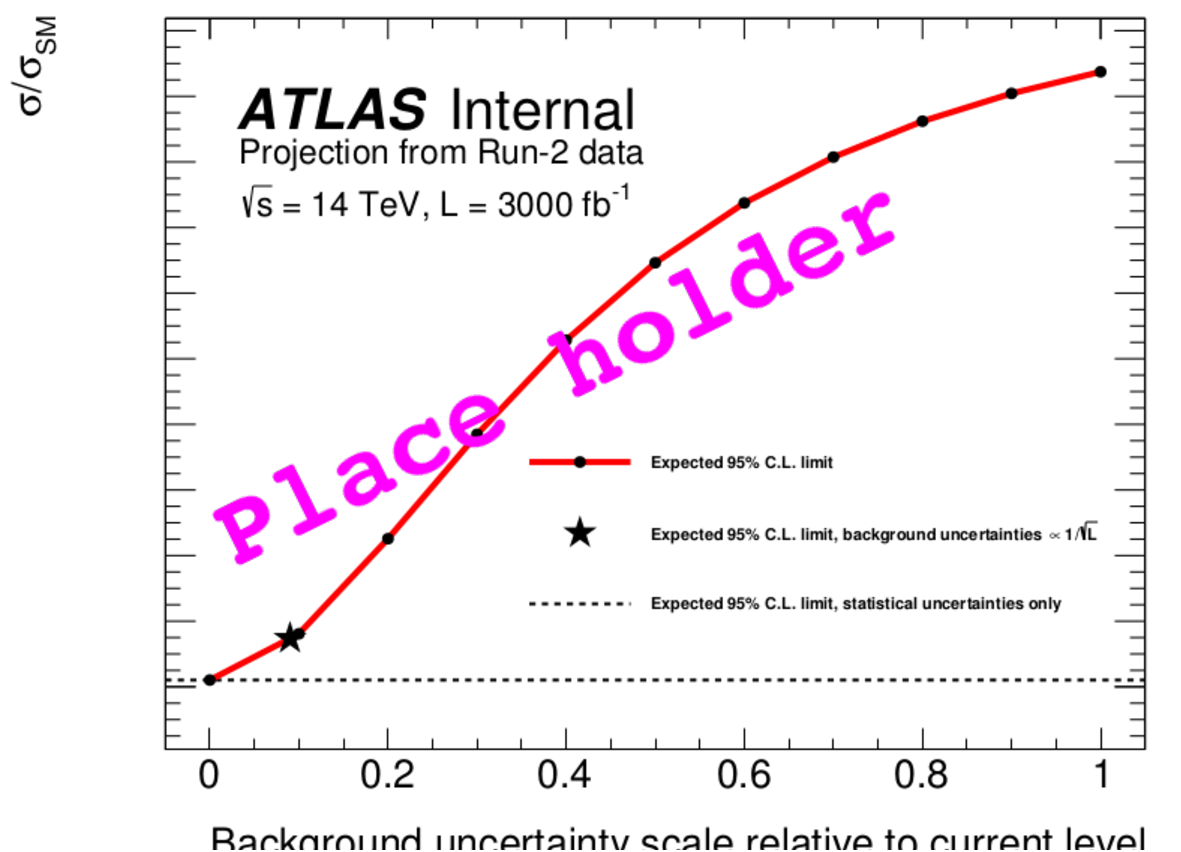
\includegraphics[width=0.5\textwidth]{\main/section3/plots/ATLAS_4b_LimitVsSyst.pdf}} 
\subfloat[]{\label{fig:ATLAS_HH_4b_b}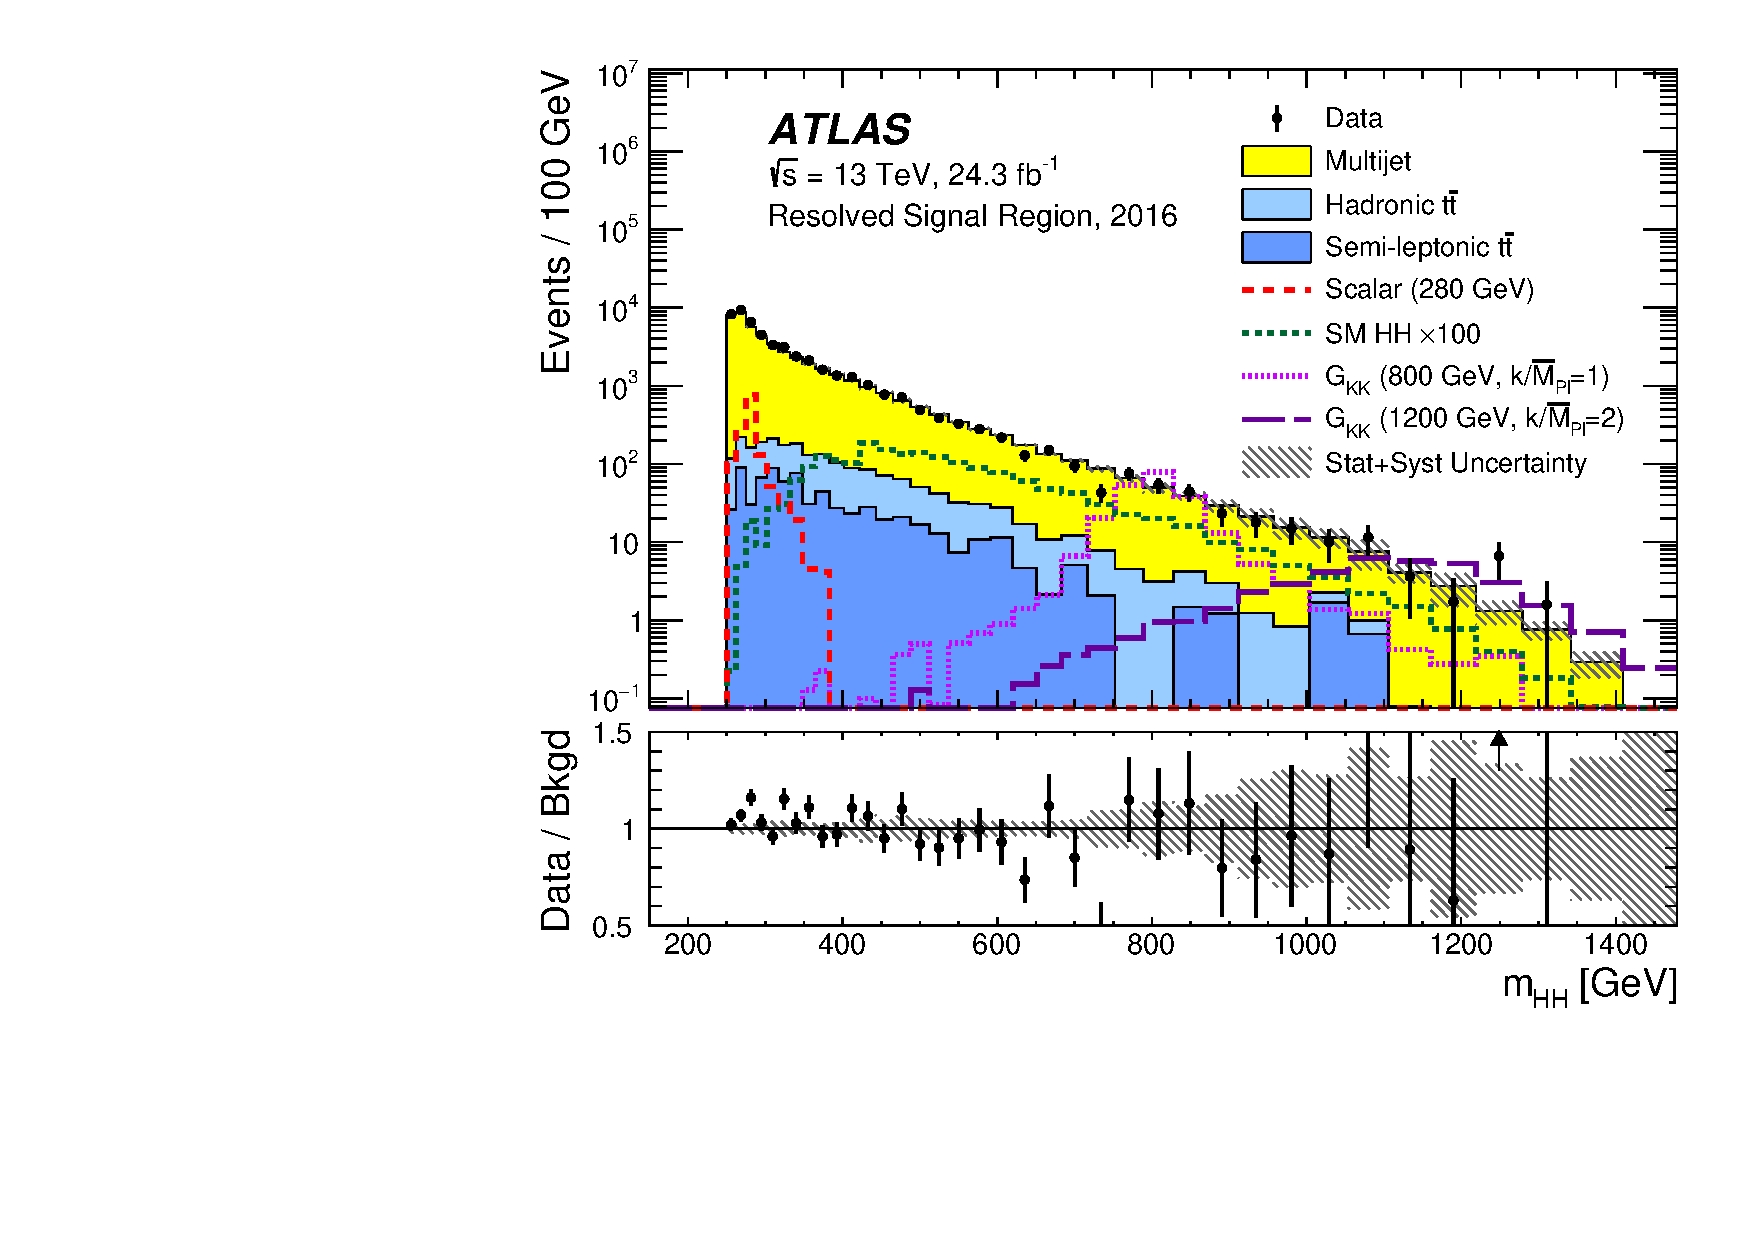
\includegraphics[width=0.5\textwidth]{\main/section3/plots/EXOT-2016-31_fig_04b.pdf}}
\caption{(a) \textcolor{red}{PLACEHOLDER} Expected 95\% Cl limit on the cross-section divided by the SM cross-section, as a function of the background modelling uncertainties. The background modelling uncertainties are each scaled by a common, constant factor relative to the 2016 uncertainties (i.e. the current uncertainties correspond to 1 here). 
The limit achievable if the uncertainties scaled proportionally to integrated luminosity is shown as the star. 
The statistical-only limit is shown as the dashed line. (b) \textcolor{red}{PLACEHOLDER} Distribution of $\mhh$ of the multijet and \ttbar\ backgrounds extrapolated to 3000~$\ifb$ of data (plot from~\cite{Aaboud:2018knk}, to be replaced).} 
\label{fig:ATLAS_HH_4b} 
\end{figure}

The final analysis discriminant, $\mhh$, showed in Figure~\ref{fig:ATLAS_HH_4b_b} is the invariant mass of the selected four-jet system, after a correction based on the known Higgs boson mass. The significance neglecting the systematic uncertainties is XX standard deviation, while it is XX standard deviation when the current systematic uncertainties are included. If the systematic uncertainty on the multijet background were scaled by the luminosity the significance would be XX standard deviations.
The high number of pile-up events at the HL-LHC cause difficulties in maintaining high acceptance when triggering on multijet final states. Ref.~\cite{Collaboration:2285584} proposes a trigger menu which thresholds corresponding to asking for jets with a transverse energy higher than 75~\UGeV. In the scenario without systematic uncertainties this would degrades the sensitivity by 50\% relative to the threshold used by default in this extrapolation.

%The allowed range at 95\% CL for $\kl$ including (without) systematic uncertainties is -4.1 -- 8.7 (-1.2 -- 8.0).

%
\paragraph{The $HH \rightarrow b\bar{b}\tau\tau$ channel}

Results~\cite{ATLASHHPUBnote} for this channel are computed by extrapolating from the Run 2 analysis of 36.1 $\ifb$ of 13~$\UTeV$ data~\cite{ATLASrun2HHbbtautau}, which currently sets the world's strongest limit by a single channel on the di-Higgs production. 
The leptonic/hadronic and hadronic/hadronic decay modes of the $\tau$-lepton are considered, the first one being separated in two categories, depending on the trigger used. A multivariate analysis with a boosted decision tree (BDT) is performed to separate the signal from the background processes. The Run-2 BDT distributions are scaled to the integrated luminosity of 3000~$\ifb$, taking into account the change of cross-section with the increased centre-of-mass energy. The binning of those BDT distributions also redefined to take into account the increased number of events.
A profile-likelihood fit is applied to the BDT score distributions shown in Figures~\ref{fig:ATLAS_HH_bbtautau_a} to~\ref{fig:ATLAS_HH_bbtautau_c}. 


\begin{figure}[!htb]
\centering 
\subfloat[]{\label{fig:ATLAS_HH_bbtautau_a}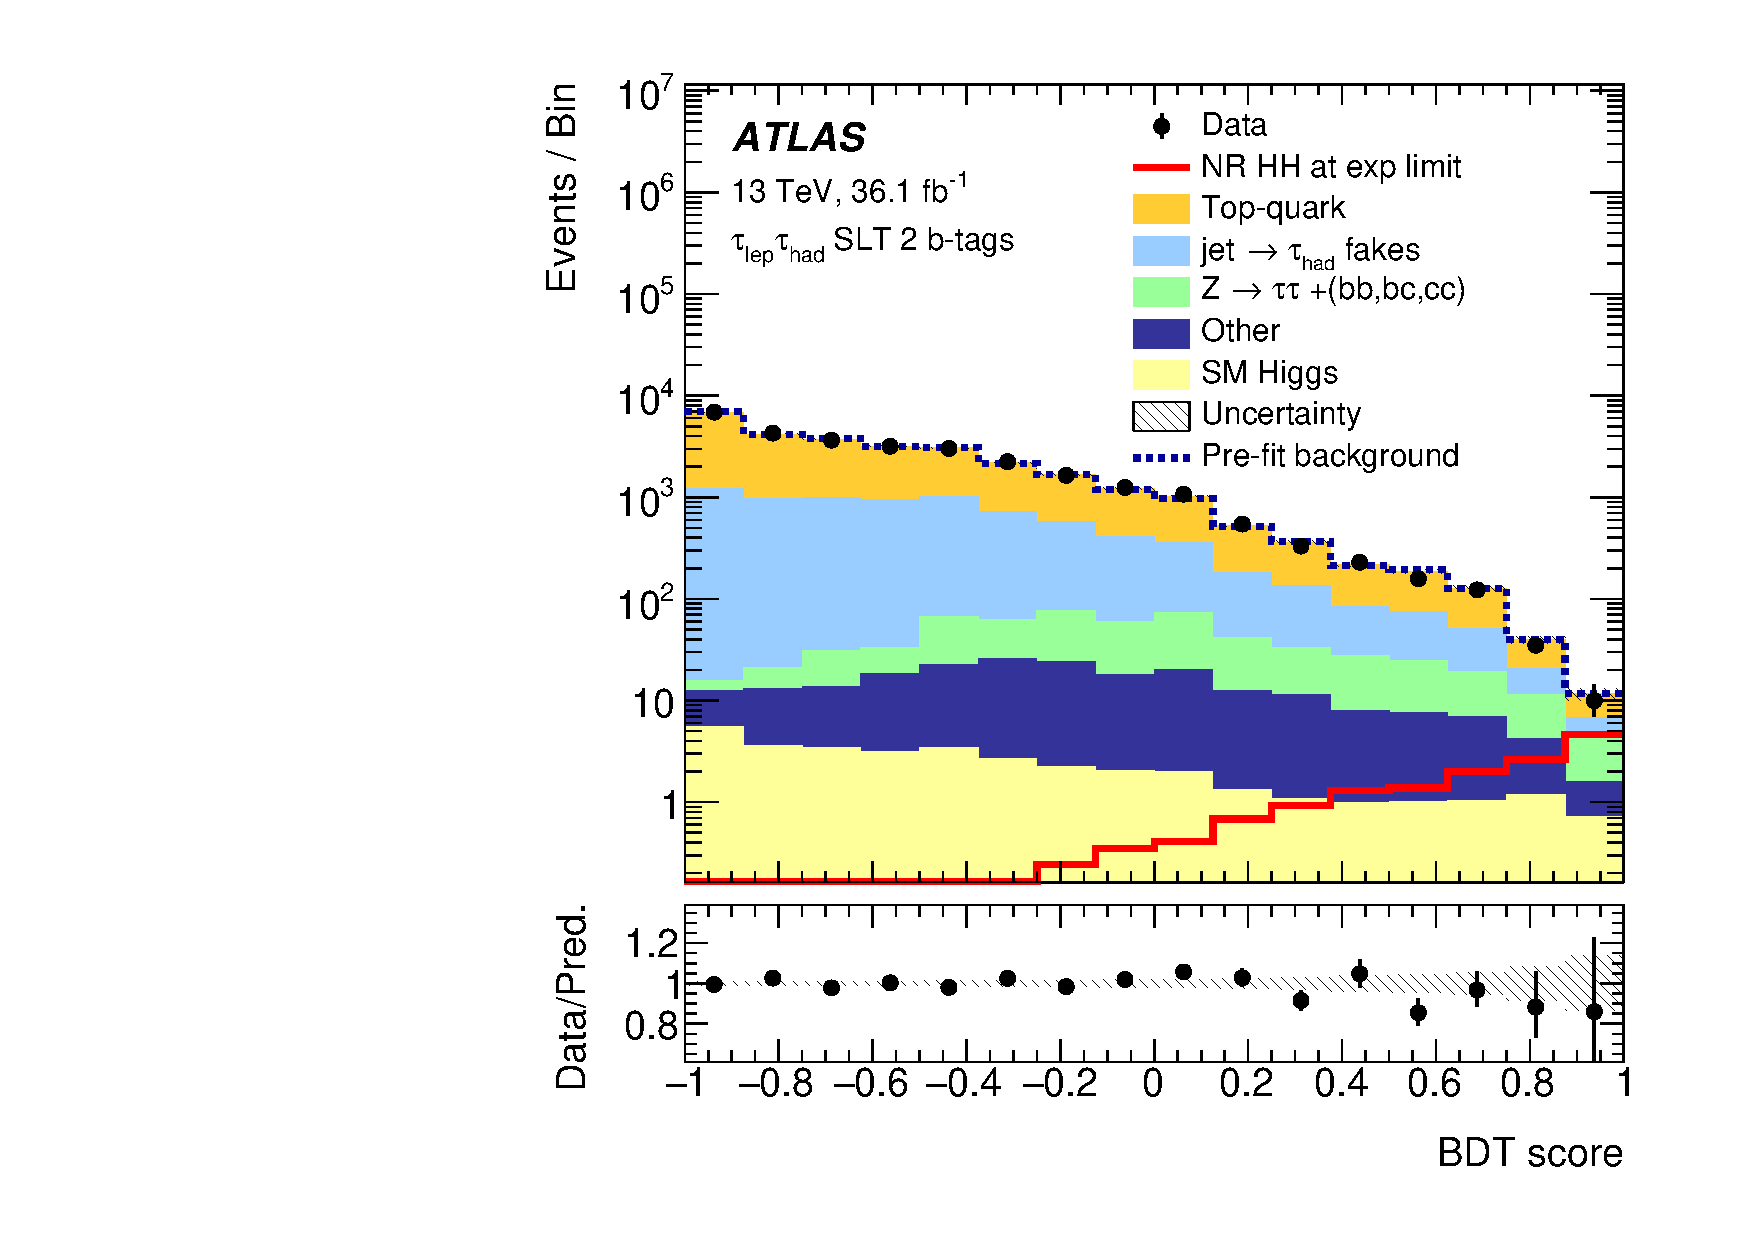
\includegraphics[width=0.5\textwidth]{\main/section3/plots/HIGG-2016-16_fig_01a.pdf}} 
\subfloat[]{\label{fig:ATLAS_HH_bbtautau_b}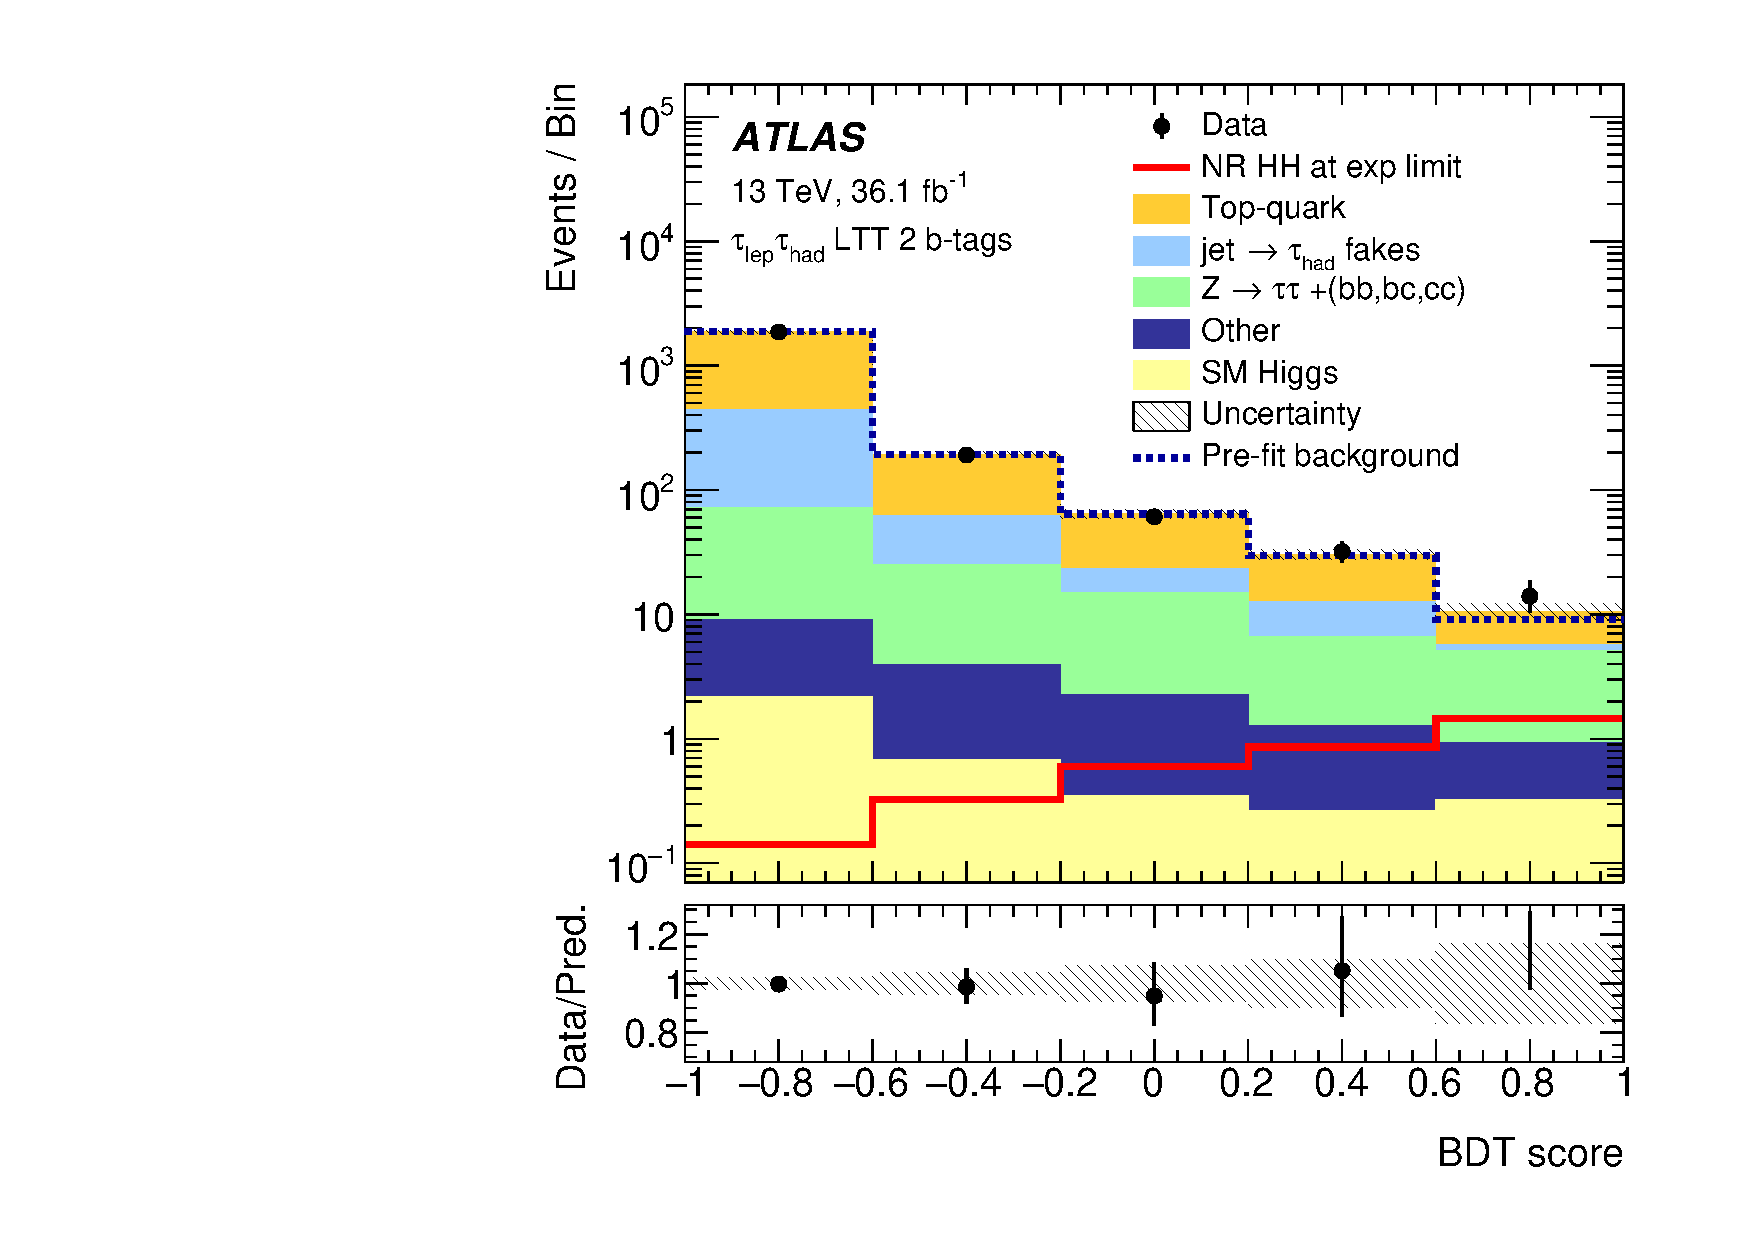
\includegraphics[width=0.5\textwidth]{\main/section3/plots/HIGG-2016-16_fig_01c.pdf}}\\
\subfloat[]{\label{fig:ATLAS_HH_bbtautau_c}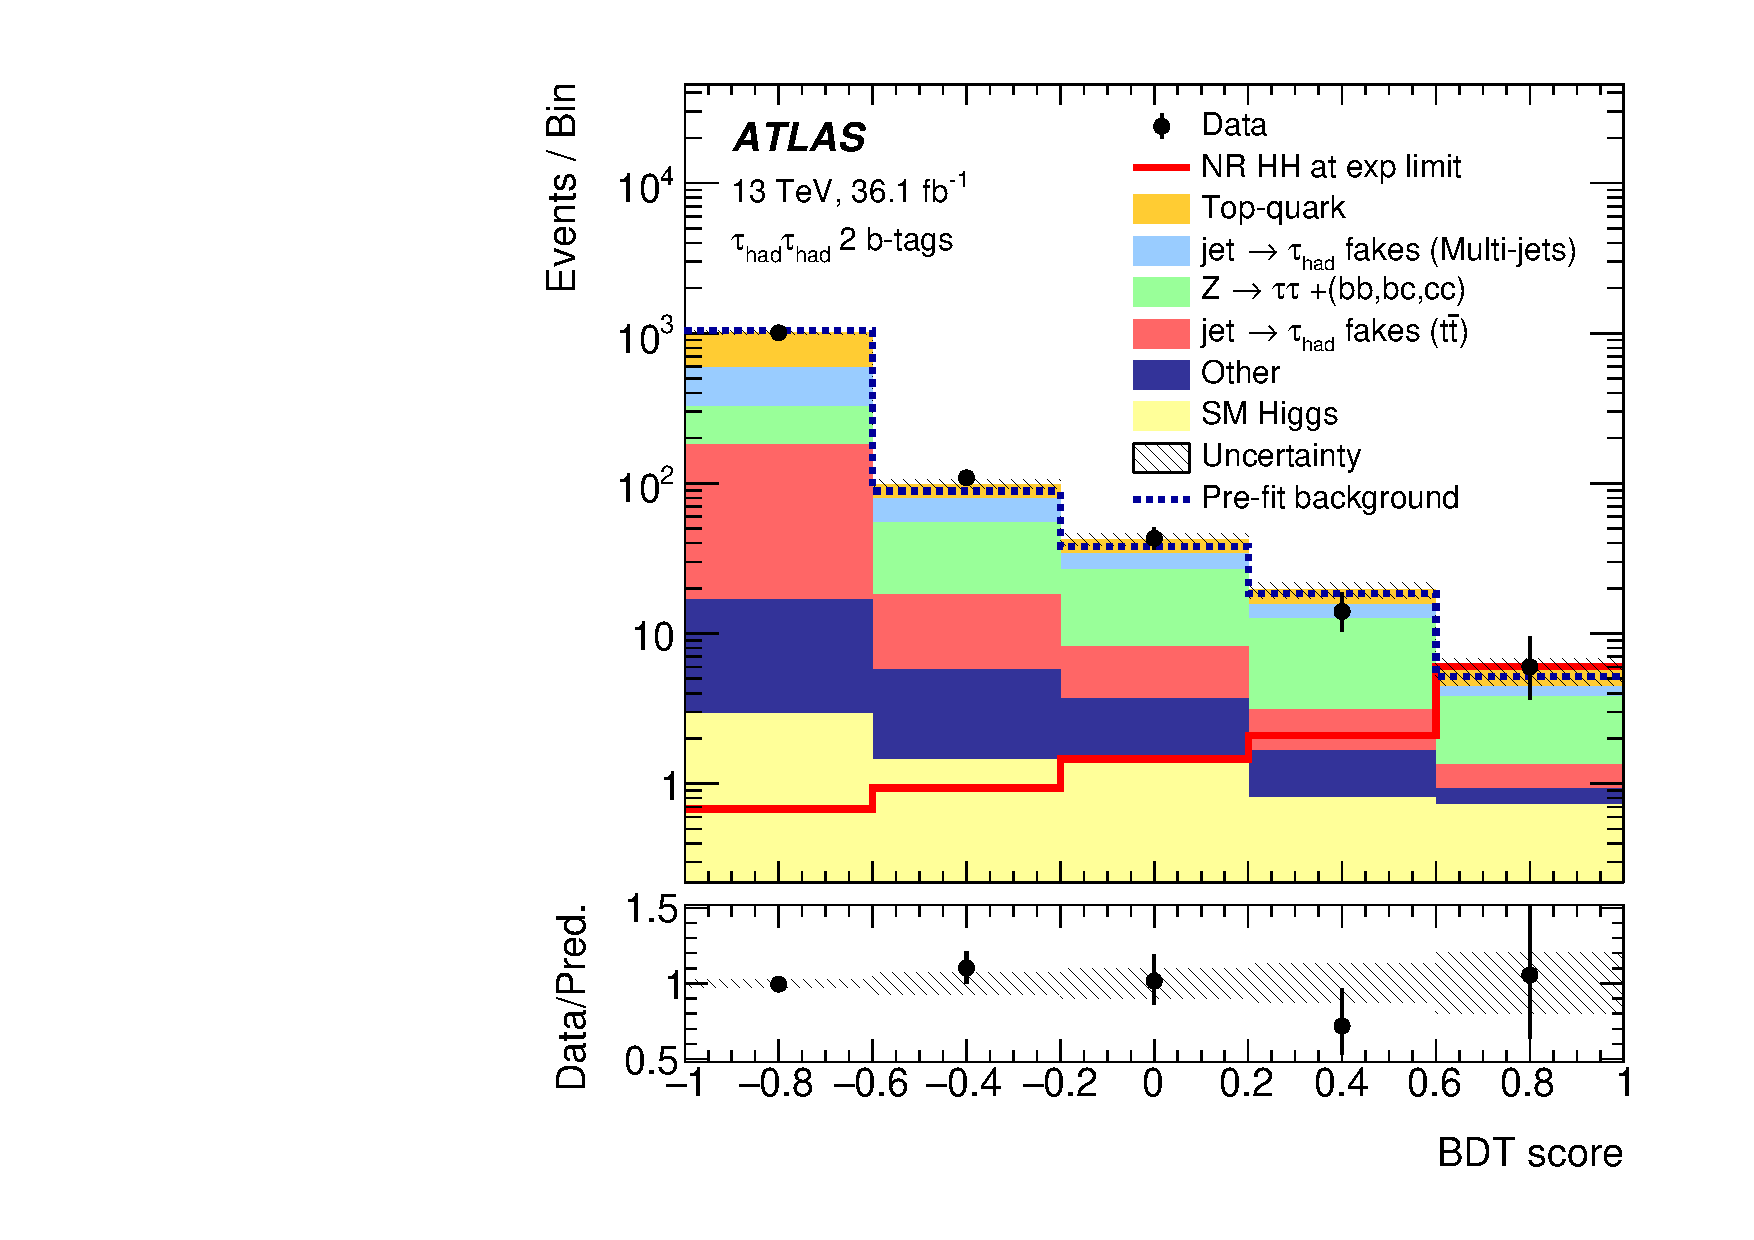
\includegraphics[width=0.5\textwidth]{\main/section3/plots/HIGG-2016-16_fig_01e.pdf}}
\subfloat[]{\label{fig:ATLAS_HH_bbtautau_d}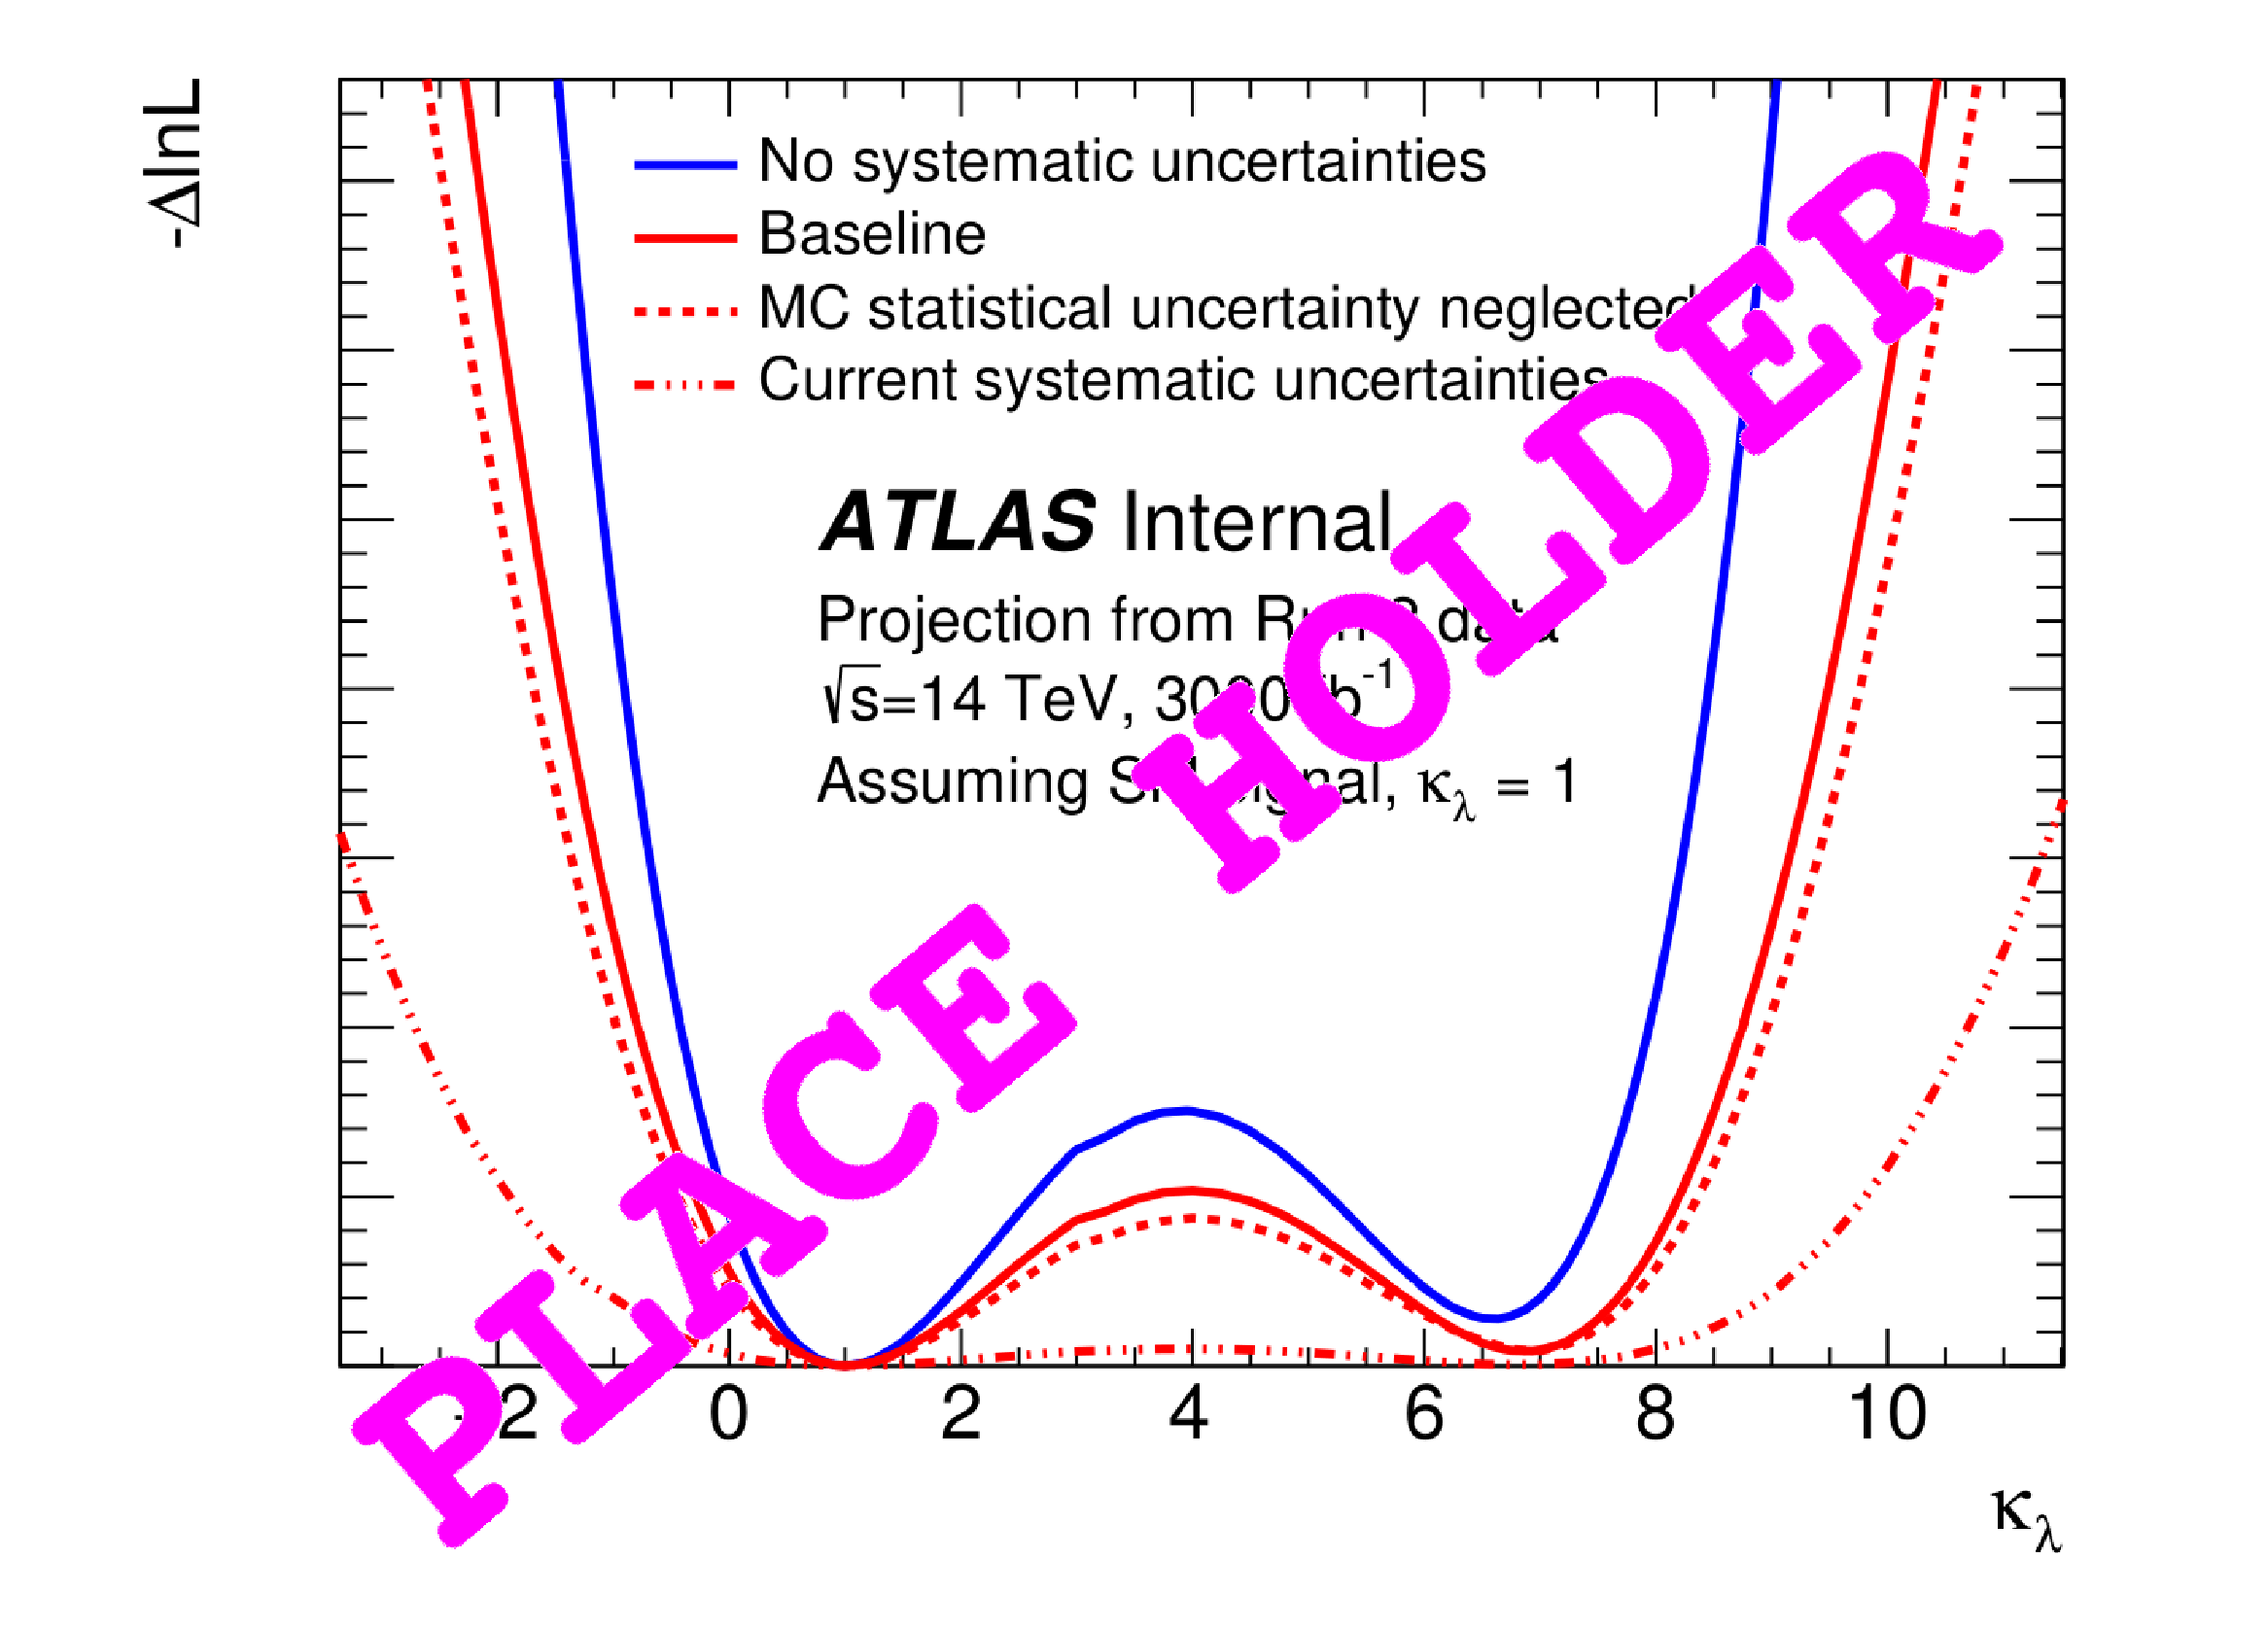
\includegraphics[width=0.5\textwidth]{\main/section3/plots/ATLAS_bbtautau_LHscan.pdf}}
\caption{(a), (b), (c) \textcolor{red}{PLACEHOLDER} Distributions of the BDT score for the three categories, extrapolated to 3000~$\ifb$ of data. The distributions are shown after the fit to the background-only hypothesis and the signal is scaled to the expected limit.  (plot from~\cite{ATLASrun2HHbbtautau}, to be replaced). (d) \textcolor{red}{PLACEHOLDER} Minimum negative-log-likelihood as a function of \kl, calculated by performing a conditional signal+backgrond fit to the background and SM signal, with different hypotheses of systematic uncertainties considered.} 
\label{fig:ATLAS_HH_bbtautau} 
\end{figure}

In the Run-2 analysis one of the dominant systematic uncertainty is the one coming from the limited statistics of the MC samples used to estimate the background. In the baseline scenario, following the prescriptions of Ref.~\cite{ATLASperformance}, this uncertainty is neglected.
Different scenarios are considered: the one in which the systematic uncertainties remain the same as for the Run-2 analysis; the scenario with the current systematic uncertainties but neglected MC statistical uncertainties and the baeline scenario for systematic uncertainties. The effect on those various scenarios is shown in Figure~\ref{fig:ATLAS_HH_bbtautau_d}.

The expected significance without systematic uncertainties is of XX standard deviations, while it is XX standard deviations when the baseline scenario for the systematic uncertainties is considered.

For the measurement of \kl\ the output score of a BDT trained on the \kl\ = 20 signal is used as the final discriminant. This was shown to provide similar performance with BDTs trained specifically for every \kl\ value, as \kl\ = 20 corresponds to a softer $\mhh$ spectrum, which is where the nominal BDT is less sensitive.
The minimum negative-log-likelihood for a SM signal hypothesis is shown in Figure~\ref{fig:ATLAS_HH_bbtautau_d}.


%A multivariate analysis with a boosted decision tree (BDT) is performed on the leptonic/hadronic and hadronic/hadronic decay modes of the $\tau$-lepton, and the BDT score is used as final discriminant. The largest systematic uncertainty of the Run 2 analysis, the simulation statistics, is neglected in the extrapolation. The expected significance of XX (XX) $\sigma$ including (without) systematics uncertainties can be achieved. The allowed range at 95\% CL for $\kl$ including (without) systematic uncertainties is XX -- XX (XX -- XX).


%
\paragraph{The $HH \rightarrow b\bar{b}\gamma\gamma$ channel}


The analysis~\cite{ATLASHHPUBnote} is based on truth level particles convoluted with the detector resolution, efficiencies and fake rates computed for $\mu$ = 200 which were extracted from fully simulated samples using the detector layout described in Ref.~\cite{ITKPixelTDR}. The selection is made using a multivariate analysis with a BDT using the full kinematic information of the event, in particular to reject the continuum and \ttH\ backgrounds. 
The diphoton invariant mass distribution, $\ensuremath{m_{\gamma\gamma}}$, is shown in Figure~\ref{fig:ATLAS_HH_bbyy_a}. The number of signal, single Higgs and continuum background in a 123-127~$\UGeV$ window is XX, XX and XX respectively.

The systematic uncertainties follow the prescriptions of Ref.~\cite{ATLASperformance}. Their effect is very small since this channel will still be dominated by statistical uncertainties at the end of the HL-LHC programm.
The expected significance was evaluated to be XX and XX standard deviations with and without systematic uncertainties.

The sensitivity of the analysis to \kl\ is assessed by using the $\mhh$ distribution for events in a 123 $ < \ensuremath{m_{\gamma\gamma}} $< 127~\UGeV. This distribution is shown in Figure~\ref{fig:ATLAS_HH_bbyy_b} for different values of \kl\ and split into eight categories. It should be noted that the BDt was trained on the SM signal only, so the constraints on \kl\ are slighlty pessimistic. Using separate BDT's trained on specific values of \kl\ ould bring negligible improvements at negative values of \kl, but up to 1$\sigma$ reduction in the expected limit at high positive values of \kl.

%The diphoton invariant mass distribution, used to extract the signal through an analytical fit, is shown in Figure~\ref{fig:ATLAS_HH_a}. The number of signal, single Higgs and continuum background in a 123-127~$\UGeV$ window is XX, XX and XX respectively, leading to a significance of XX (XX)$\sigma$ including (without) systematics uncertainties. The allowed range at 95\% CL for $\kl$ including (without) systematic uncertainties is XX -- XX (XX -- XX).


\begin{figure}[!htb]
\centering 
\subfloat[]{\label{fig:ATLAS_HH_bbyy_a}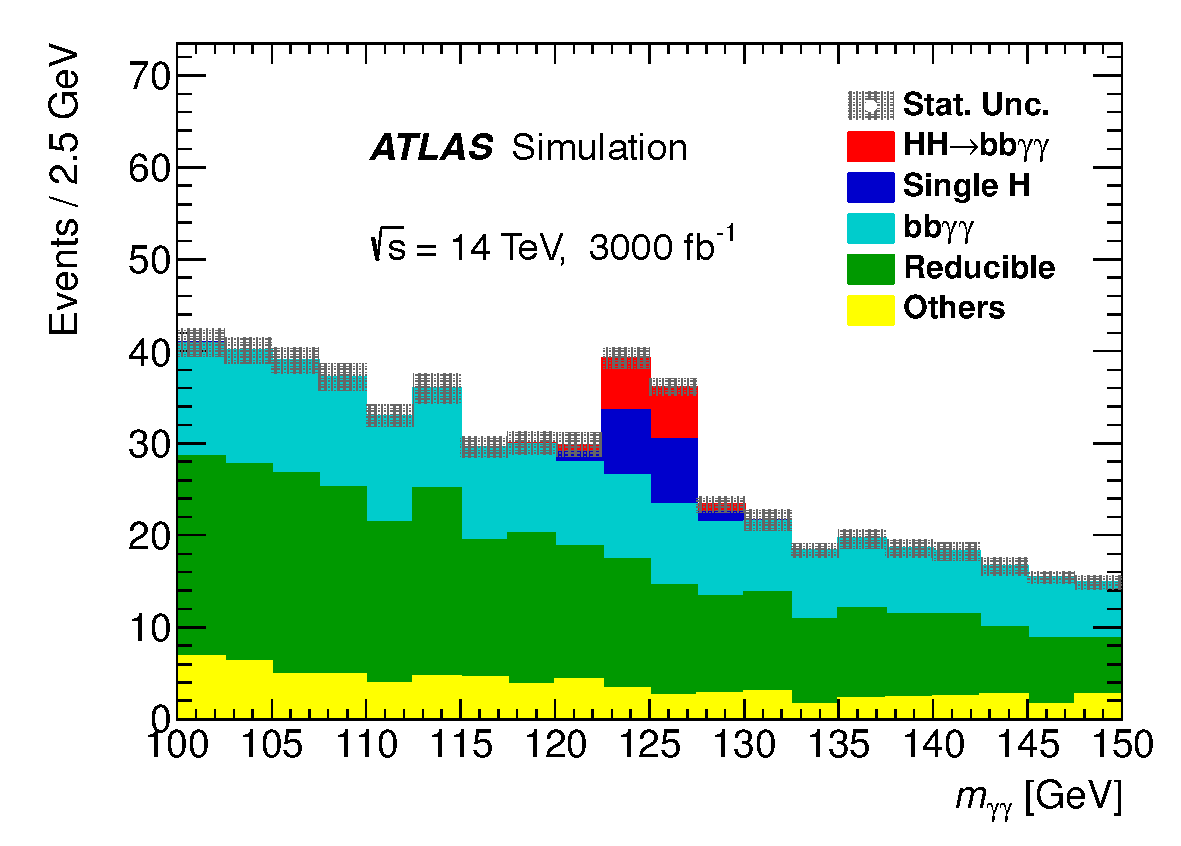
\includegraphics[width=0.5\textwidth]{\main/section3/plots/ch03_fig_033.pdf}} 
\subfloat[]{\label{fig:ATLAS_HH_bbyy_b}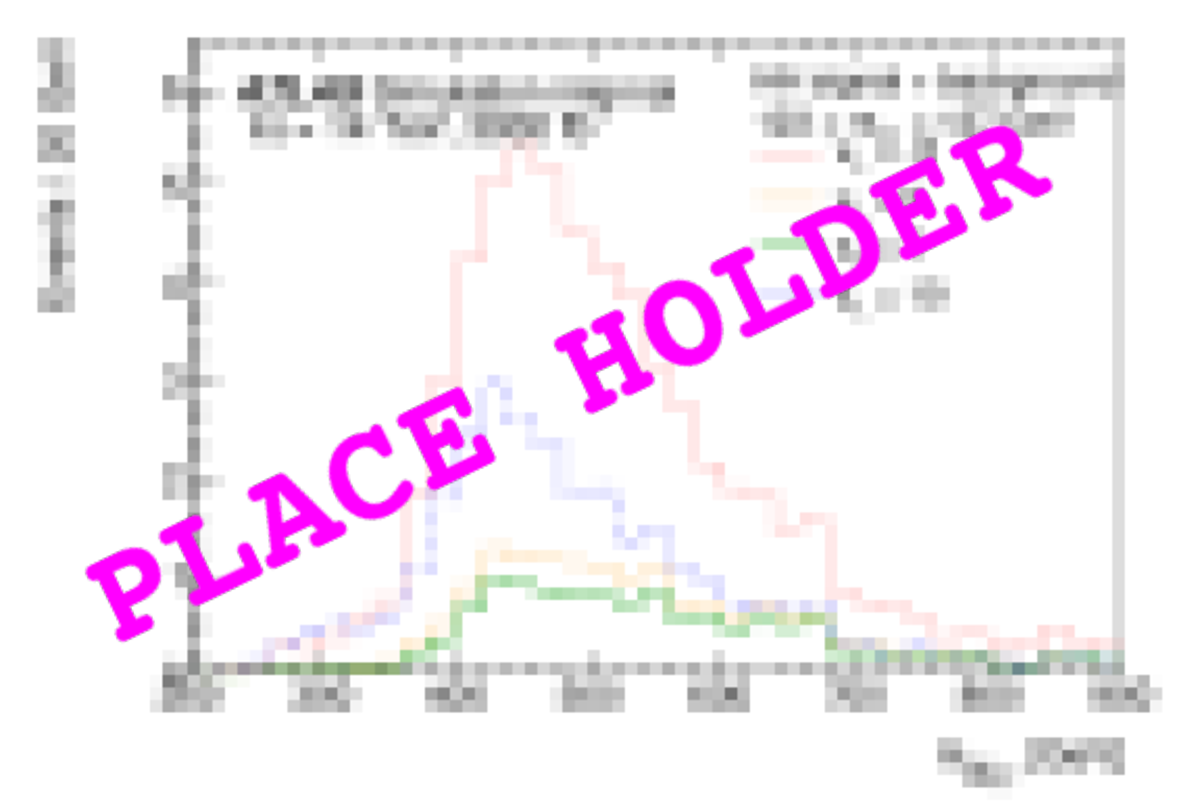
\includegraphics[width=0.5\textwidth]{\main/section3/plots/mbbyy_SignalBackground_20GeVbins_variouskappa.pdf}} 
\caption{(a)\textcolor{red}{PLACEHOLDER} Diphoton invariant mass distribution after selection, for the Standard Model HH signal and different backgrounds (plot from~\cite{ITKPixelTDR}, to be replaced). (b) \textcolor{red}{PLACEHOLDER} Invariant mass of the $b\bar{b}\gamma\gamma$ system after selection and a 123 $ < \ensuremath{m_{\gamma\gamma}} $< 127~\UGeV cut for the sum of the signal and the background. The different lines correspond to different values of \kl.} 
\label{fig:ATLAS_HH_bbyy} 
\end{figure}


%
\paragraph{Combined results}


The combination of various channels is realised by constructing a combined likelihood function that takes into account data, models and correlated systematic uncertainties from all channels. 

Setting appropriate nuisance parameters (NP) to be correlated with one another induced a negligible change in the combination results compared to assuming all nuisance parameters are uncorrelated. No strong correlation between any of the NP are found by the fits, with the exception of some correlation between the background models of the $b\bar{b}b\bar{b}$ and $b\bar{b}\tau\tau$ channels. Theoretical uncertainties on the cross-sections have negligible impact on the combined results.

The combined significance is XX and XX standard deviations with and without systematic uncertainties included.

The combined sensitivity of the three channels to \kl\ is assessed by generating an Asimov dataset containing the background plus SM signal. The ratio of the negative-log-likelihood of the maximum likelihood fit for \kl\ was calculated and shown in Figure~\ref{fig:ATLAS_HH_comb}. A morphing technique~\cite{ATL-PHYS-PUB-2015-047} is used to generate signal distributions of $\mhh$ for any arbitrary value of \kl.

\begin{figure}[!htb]
\centering 
\subfloat[statistical uncertainties only]{\label{fig:ATLAS_HH_comb_a}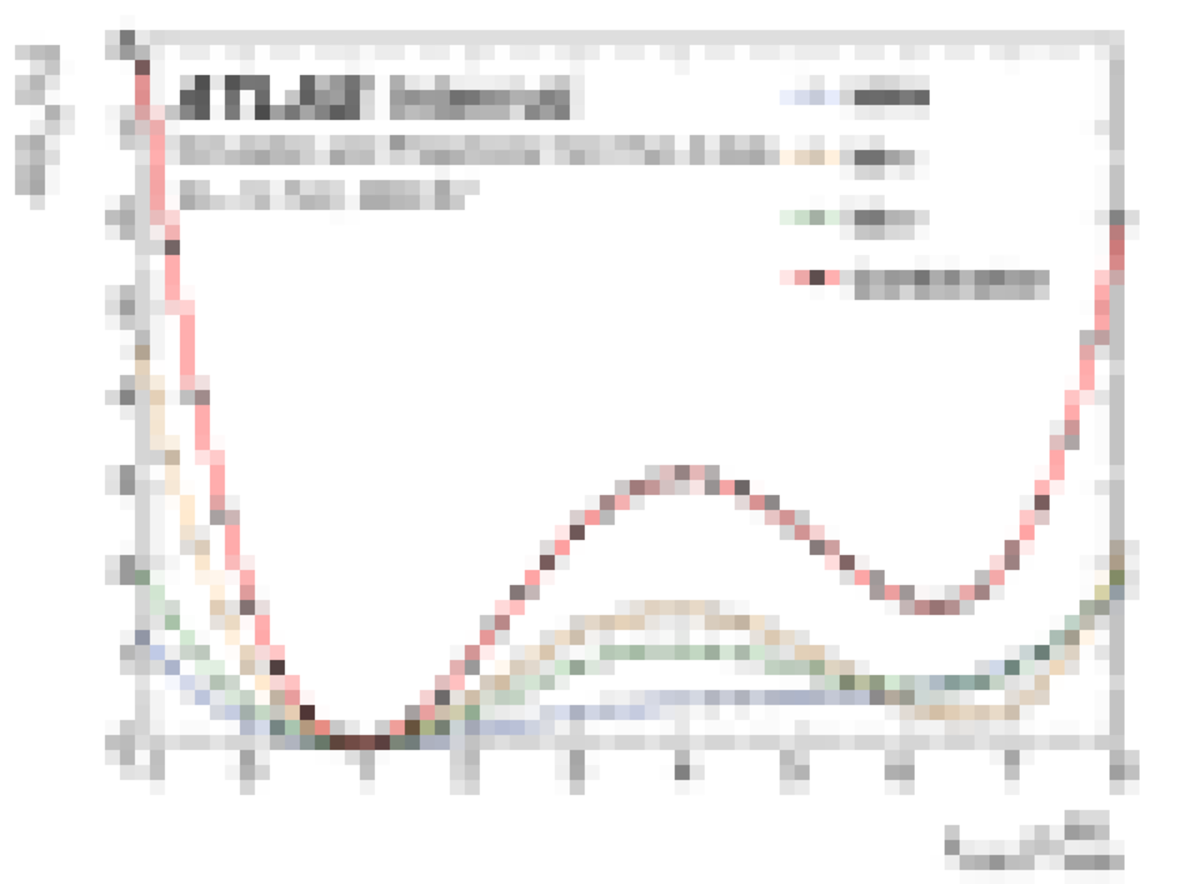
\includegraphics[width=0.5\textwidth]{\main/section3/plots/bbbb_bbtt_bbyy_lHHH0100_NoSyst_overlay_Internal.pdf}} 
\subfloat[systematic uncertainties included]{\label{fig:ATLAS_HH_comb_b}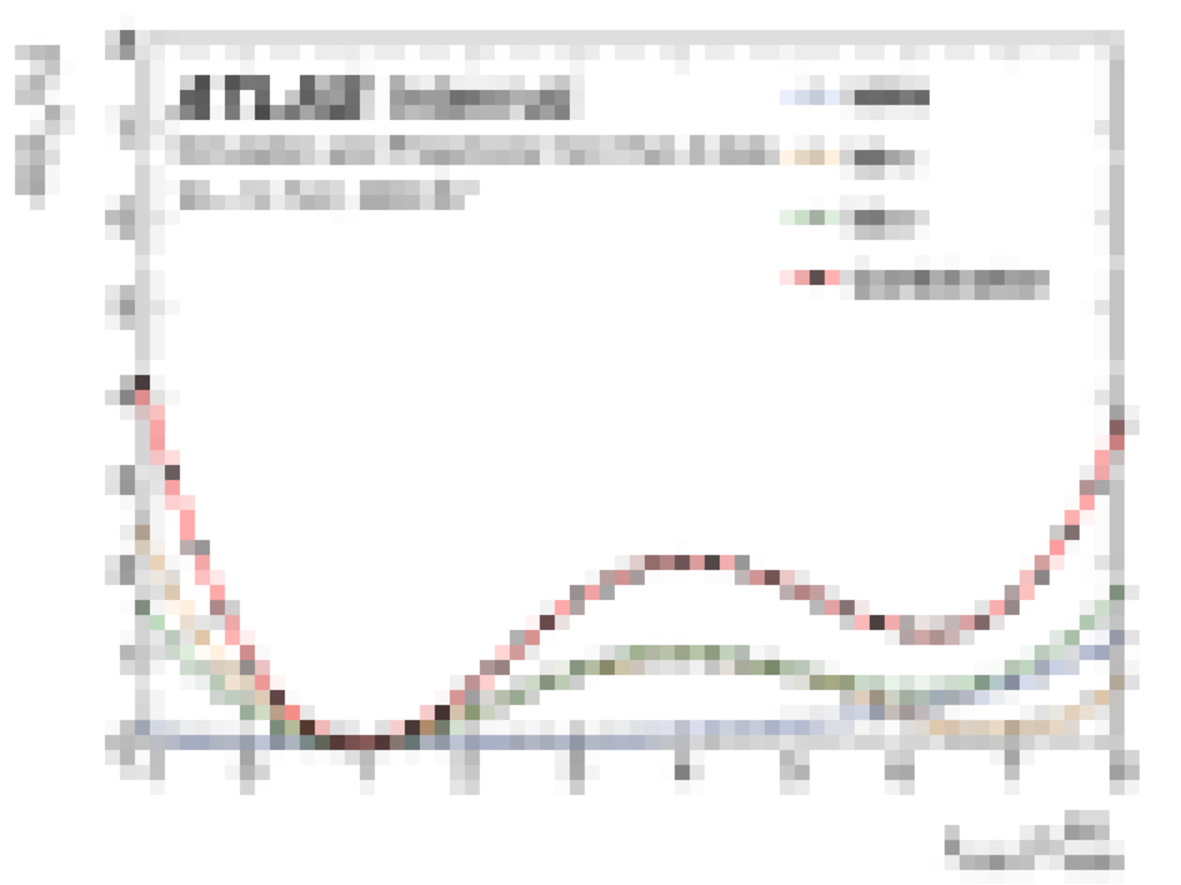
\includegraphics[width=0.5\textwidth]{\main/section3/plots/bbbb_bbtt_bbyy_lHHH0100_AllSyst_overlay_Internal.pdf}} 
\caption{Minimum negative-log-likelihood as a function of \kl, calculated by performing a conditional signal+backgrond fit to the background and SM signal with (a)\textcolor{red}{PLACEHOLDER} only statistical uncertainties (b) \textcolor{red}{PLACEHOLDER} systematic uncertainties included. The solid line show the results for the combination, while the empty shapes correspond to the individual channels. The dashed lines at $-ln(L_{H}/L_{0})$ = 0.5 and 2 indicates the values corresponding to a 1~$\sigma$ and 2~$\sigma$ confidence interval respectively (assuming an asymptotic $\chi^{2}$ distribution of the test statistics).} 
\label{fig:ATLAS_HH_comb} 
\end{figure}

%The 68\% Confidence Intervals are $XX \leq \kl\ \leq XX$ and $XX \leq \kl\ \leq XX$ with and without systematic uncertainties respectively. 
The trilinear coupling modifier is measured to be:
%\begin{equation}
\[
\begin{split}
1^{+XX}_{-XX} [^{+XX}_{-XX} (stat) ^{+XX}_{-XX} (syst)] \text{ at 68\% CL} \\
1^{+XX}_{-XX} [^{+XX}_{-XX} (stat) ^{+XX}_{-XX} (syst)] \text{ at 95\% CL}
\end{split}
%\end{equation}
\]

Assuming the SM HH signal the expected exclusion significance for the \kl\ = 0 hypothesis, i.e. no Higgs self-coupling, is XX and XX standard deviations with and without systematic uncertainties respectively.








%The combination of the three decay channels leads to an expected significance of XX (XX)$\sigma$ including (without) systematics uncertainties~\cite{ATLASHHPUBnote}. The 95\% CL upper limit on the HH production cross-section is shown in Figure~\ref{fig:ATLAS_HH_b}. The allowed range at 95\% CL for $\kl$ including (without) systematic uncertainties is XX -- XX (XX -- XX). A measurement of \lHHH\ is also performed, improved by the use of the $m_{HH}$ shape in the $HH \rightarrow b\bar{b}b\bar{b}$ and $HH \rightarrow b\bar{b}\gamma\gamma$ analyses. 


